\section{Activity Analysis}

% Note: activity SAGs can go beyond friends.

In this section we evaluate the correlation between the conditional
entropy and size of groups, pages and favourites.
\begin{itemize}
  \item Fig \ref{Fig3} shows the relationship between conditional
    entropy/logistic regression weights and size of activity
    groups. It shows that the activity groups of small size can be
    highly predictive whereas large groups are rarely predictive.
  \item In \ref{Fig4} we plot the average conditional entropy of top
    10\% features cumulative over the size of activity group. It
    distinctly shows that the small sized group, pages and favourites
    have low average conditional entropy. Furthermore, it explains
    average conditional entropy decreases as size increases. From the
    figure \ref{Fig4} we can infer that the group size upto 50 and
    page/favourite size upto $10^{5}$ can be highly predictive.
  \item We also analyze predictiveness of favourites by categories in
    fig \ref{Fig5}. It shows that television, books, music and movies
    are predictive whereas favourite teams, sports and athletes are
    less predictive.
\end{itemize}


%%%%%%%%%%%%%%%%%%%%%%%%%%%%%%%%%%%%%%%%%%%%%%%%%%%%%%%%%%%%%%%%%%%%%%%%%%%
\begin{figure*}[h]
\centering
\begin{tabular}{ccc}
\subfloat[Fig:][]{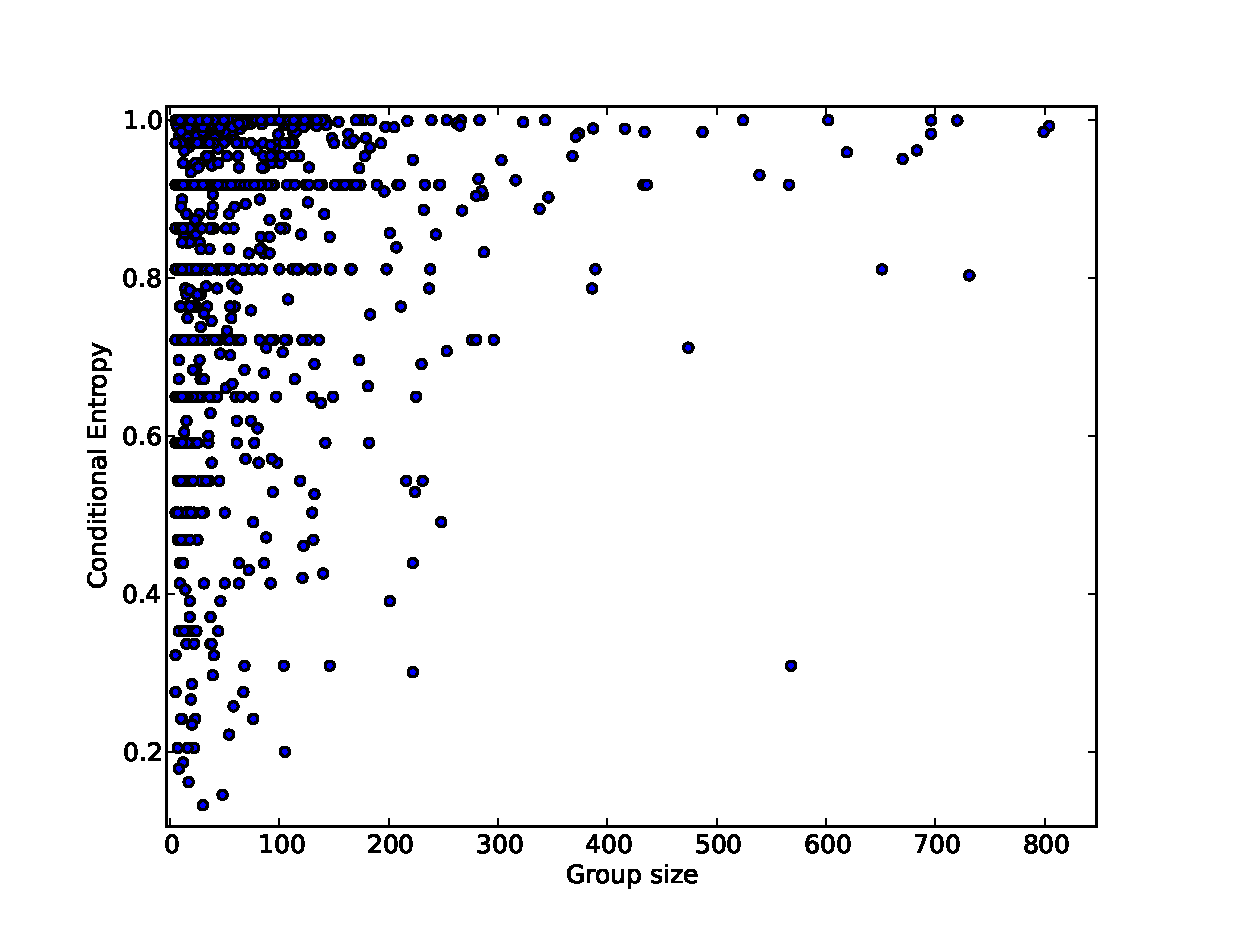
\includegraphics[width=40mm, height=25mm]{data/plots/scatterplots/vssize/CEvsGroupSize.eps}}
\subfloat[Fig:][]{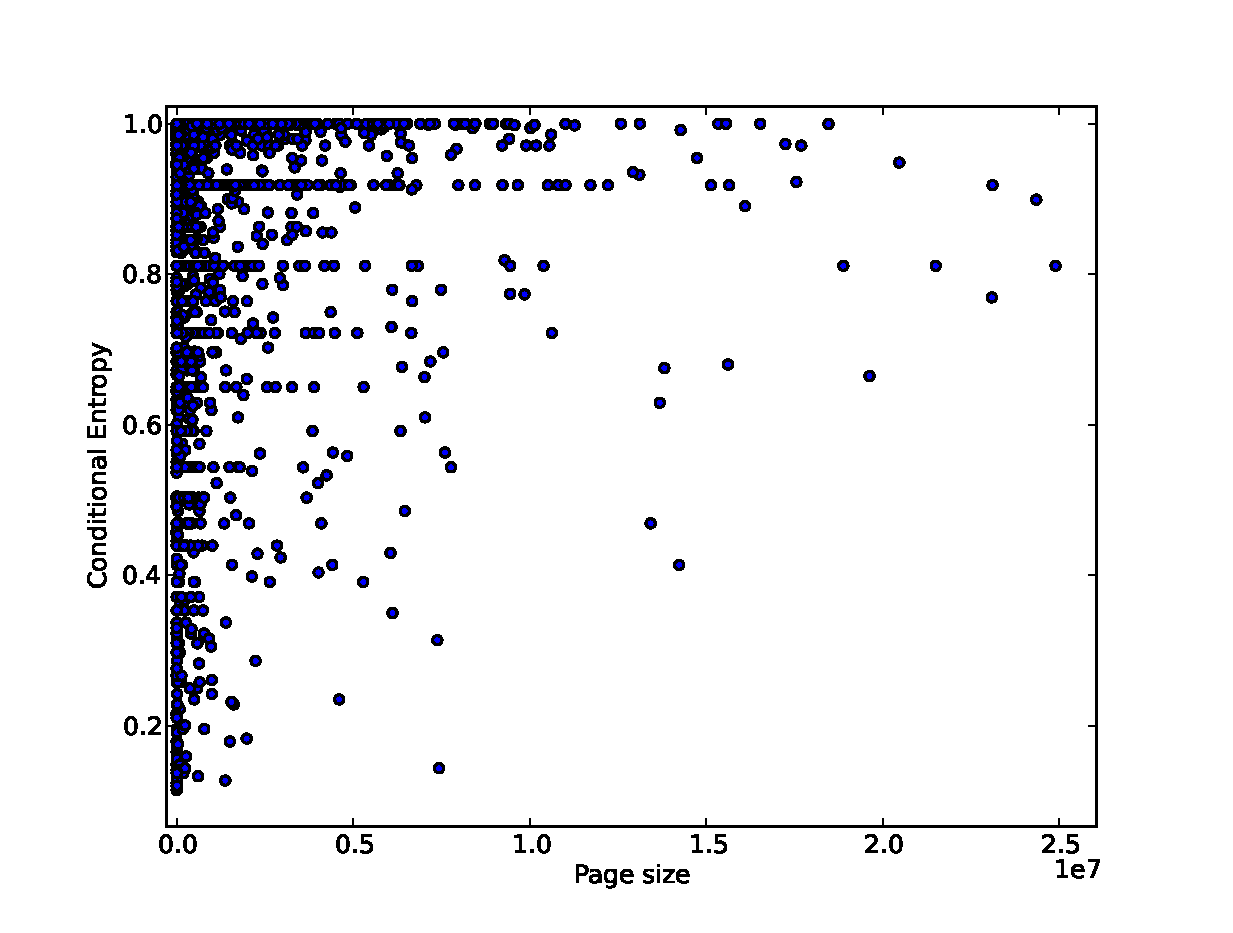
\includegraphics[width=40mm, height=25mm]{data/plots/scatterplots/vssize/CEvsPageSize.eps}}
\subfloat[Fig:][]{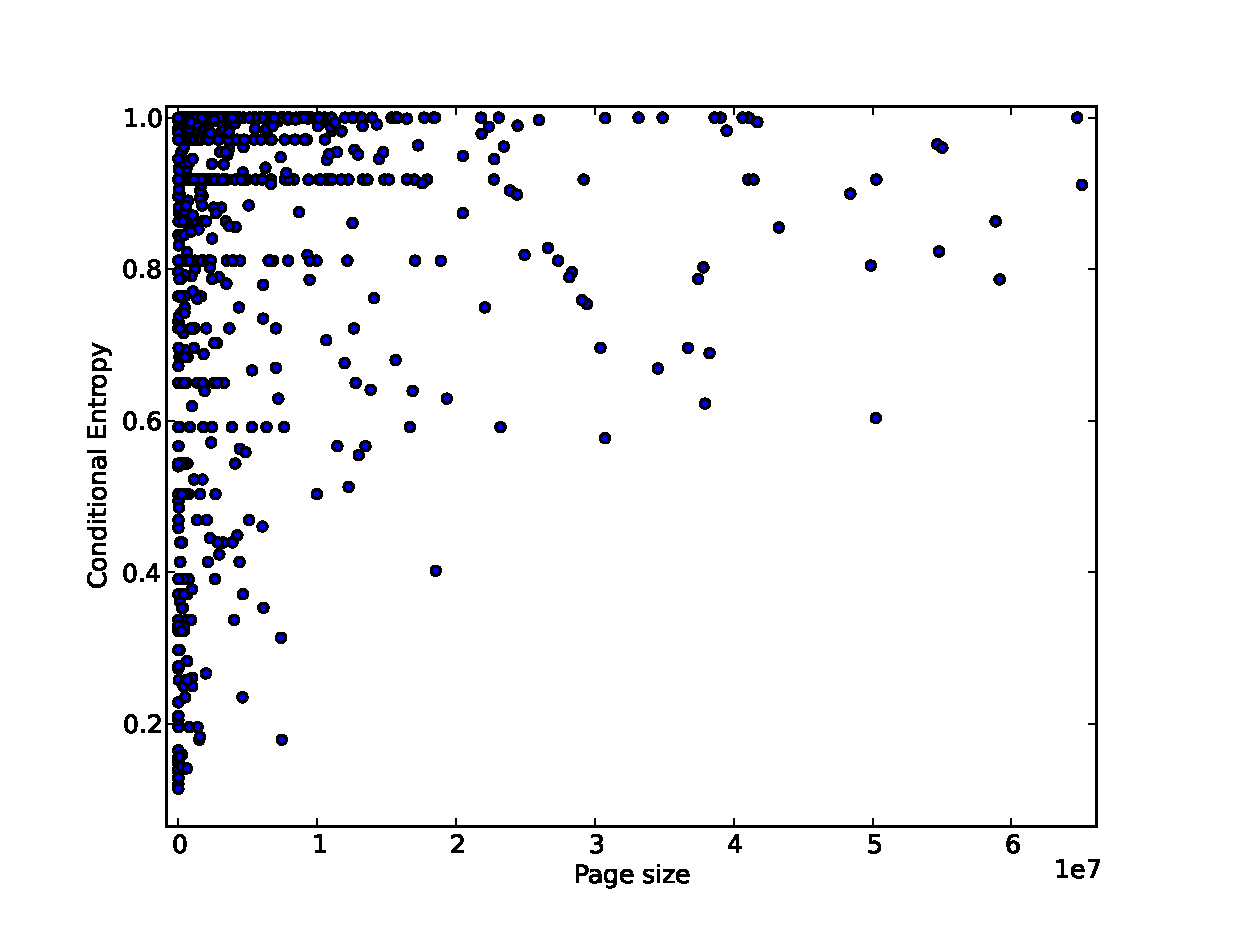
\includegraphics[width=40mm, height=25mm]{data/plots/scatterplots/vssize/CEvsFavSize.eps}} \\
\subfloat[Fig:][]{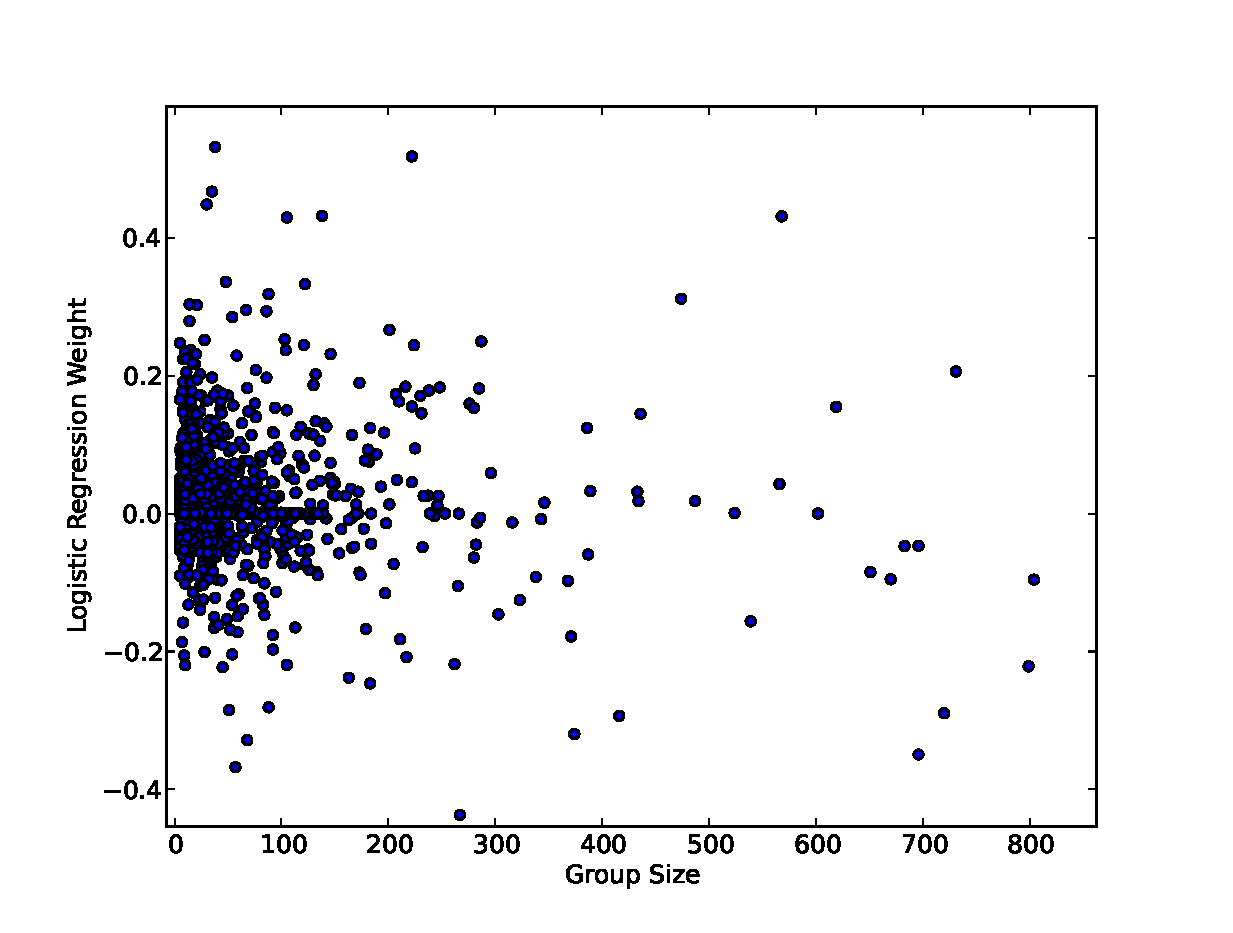
\includegraphics[width=40mm, height=25mm]{data/plots/scatterplots/LRweights/LRweightvsGroupSize.eps}}
\subfloat[Fig:][]{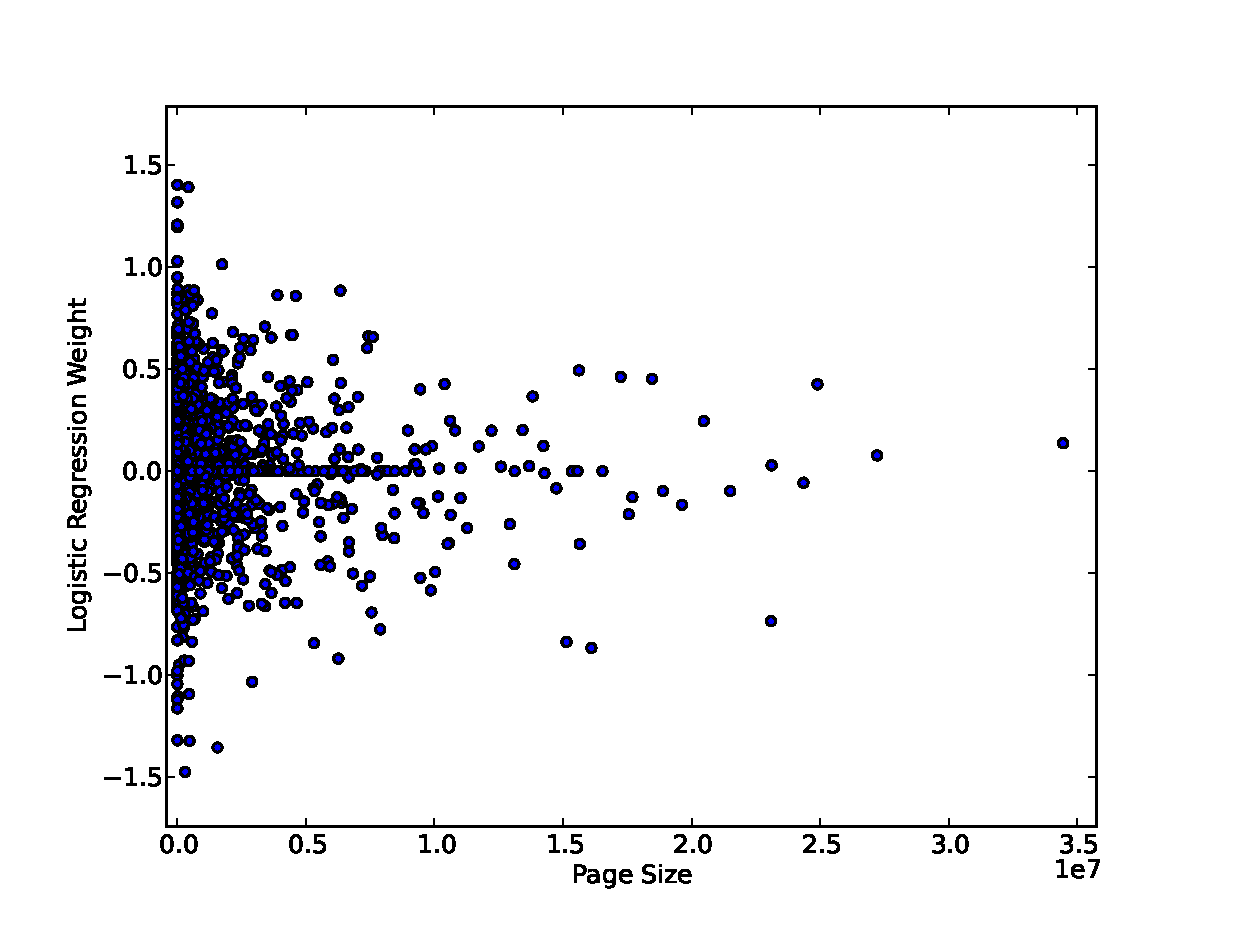
\includegraphics[width=40mm, height=25mm]{data/plots/scatterplots/LRweights/LRweightvsPageSize.eps}}
\subfloat[Fig:][]{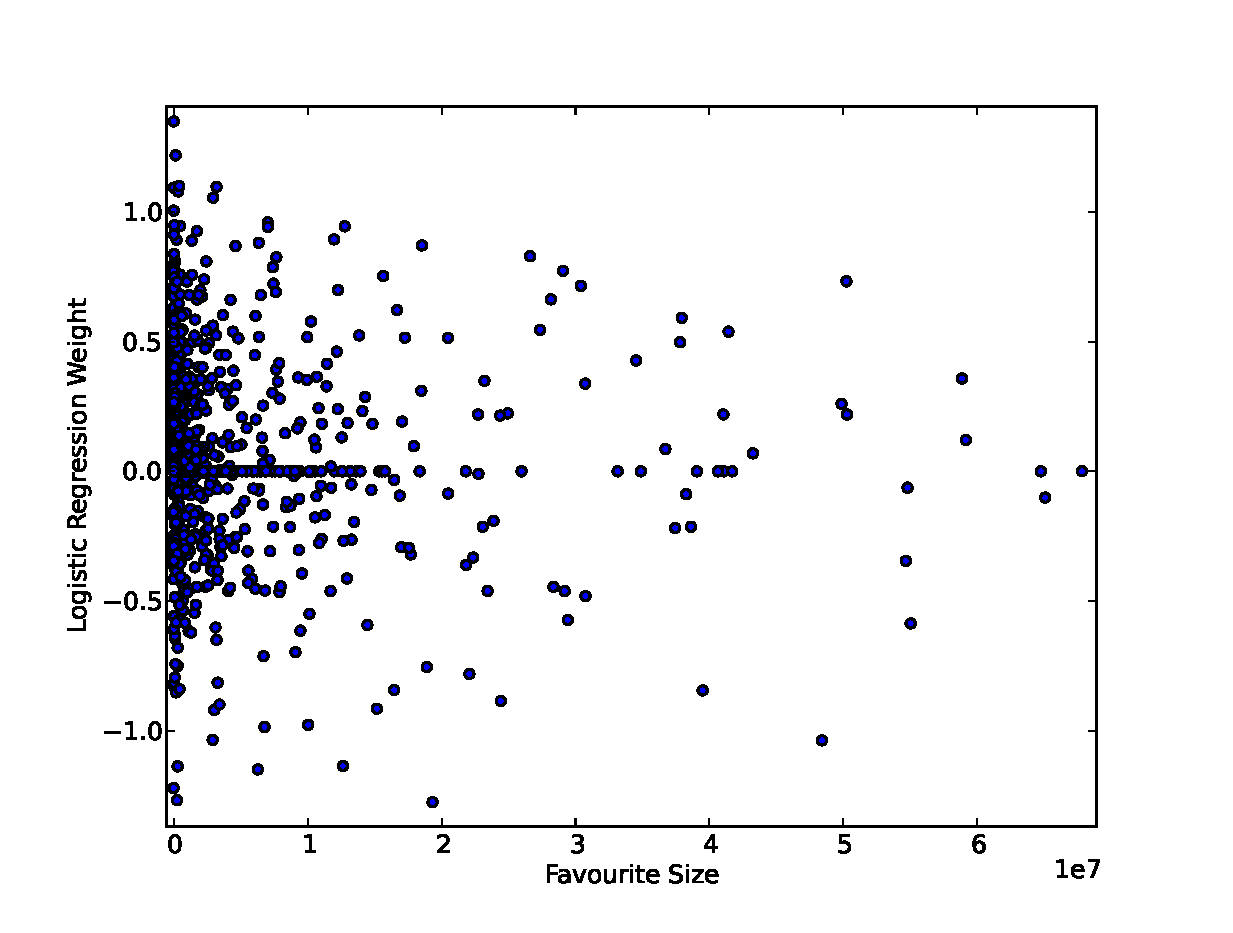
\includegraphics[width=40mm, height=25mm]{data/plots/scatterplots/LRweights/LRweightvsFavouriteSize.eps}} \\
\end{tabular}
\caption {Conditional entropy vs size (a-c); logistic regression feature weights vs size (d-f) }
\label{Fig3}
\end{figure*}
%%%%%%%%%%%%%%%%%%%%%%%%%%%%%%%%%%%%%%%%%%%%%%%%%%%%%%%%%%%%%%%%%%%%%%%%%%%

%%%%%%%%%%%%%%%%%%%%%%%%%%%%%%%%%%%%%%%%%%%%%%%%%%%%%%%%%%%%%%%%%%%%%%%%%%%
\begin{figure*}[h]
\centering
\begin{tabular}{ccc}
\subfloat[Fig: ][]{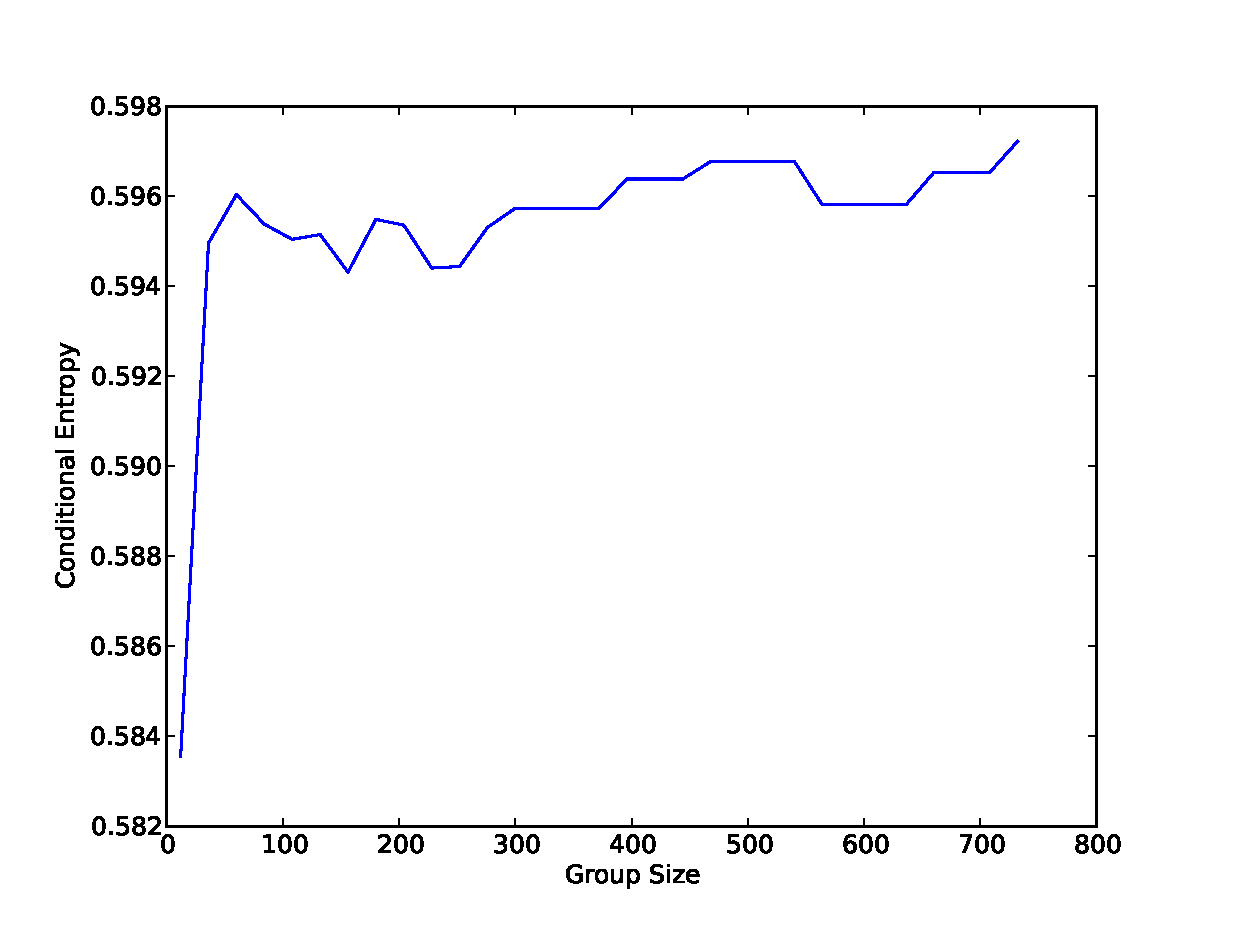
\includegraphics[scale=0.25]{data/plots/cumulativeEntropy/CEvsGroupSize_Top300Features_30bins.eps}}
\subfloat[Fig: ][]{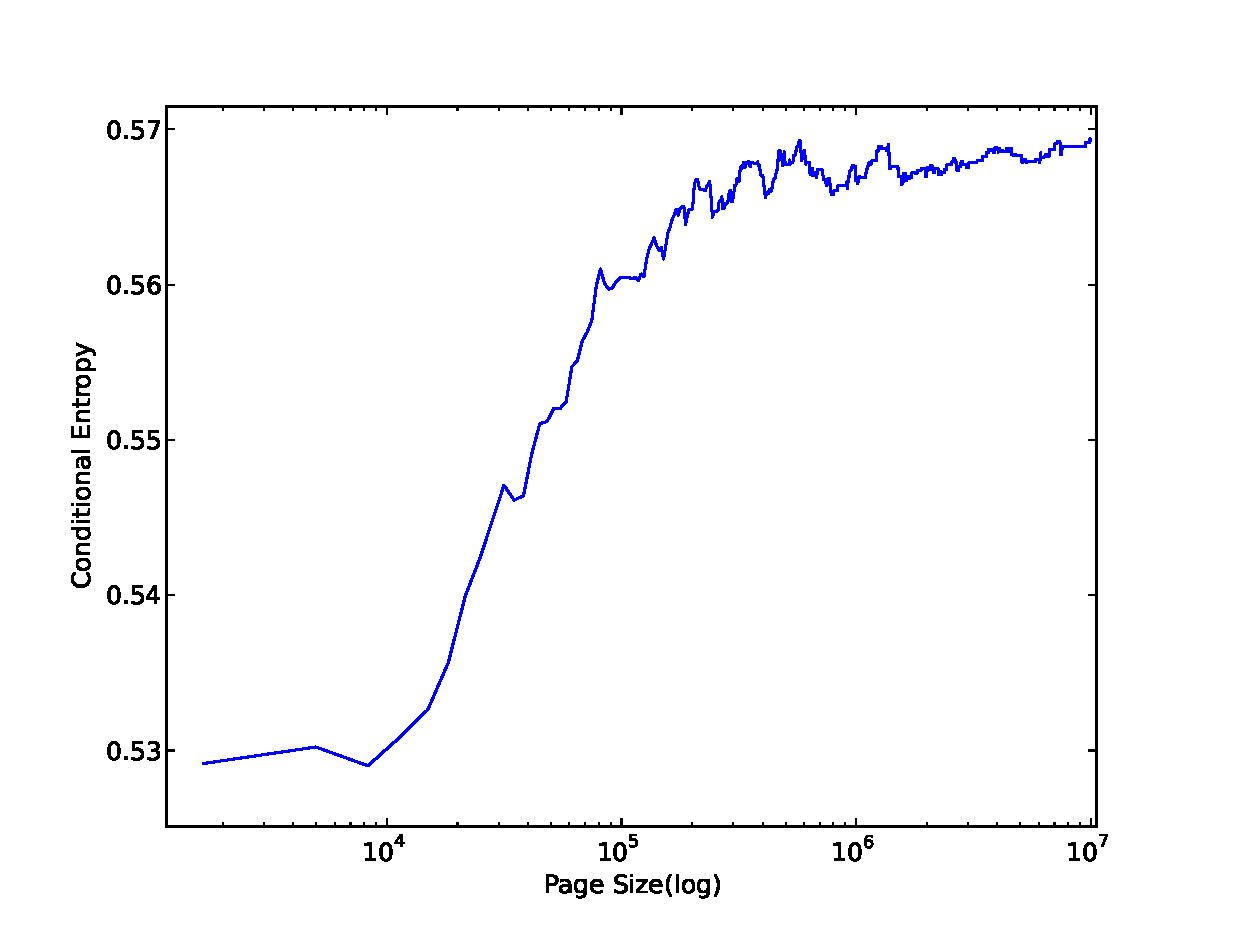
\includegraphics[scale=0.25]{data/plots/cumulativeEntropy/CEvsPageSize_Top800Features_3000bins.eps}}
\subfloat[Fig: ][]{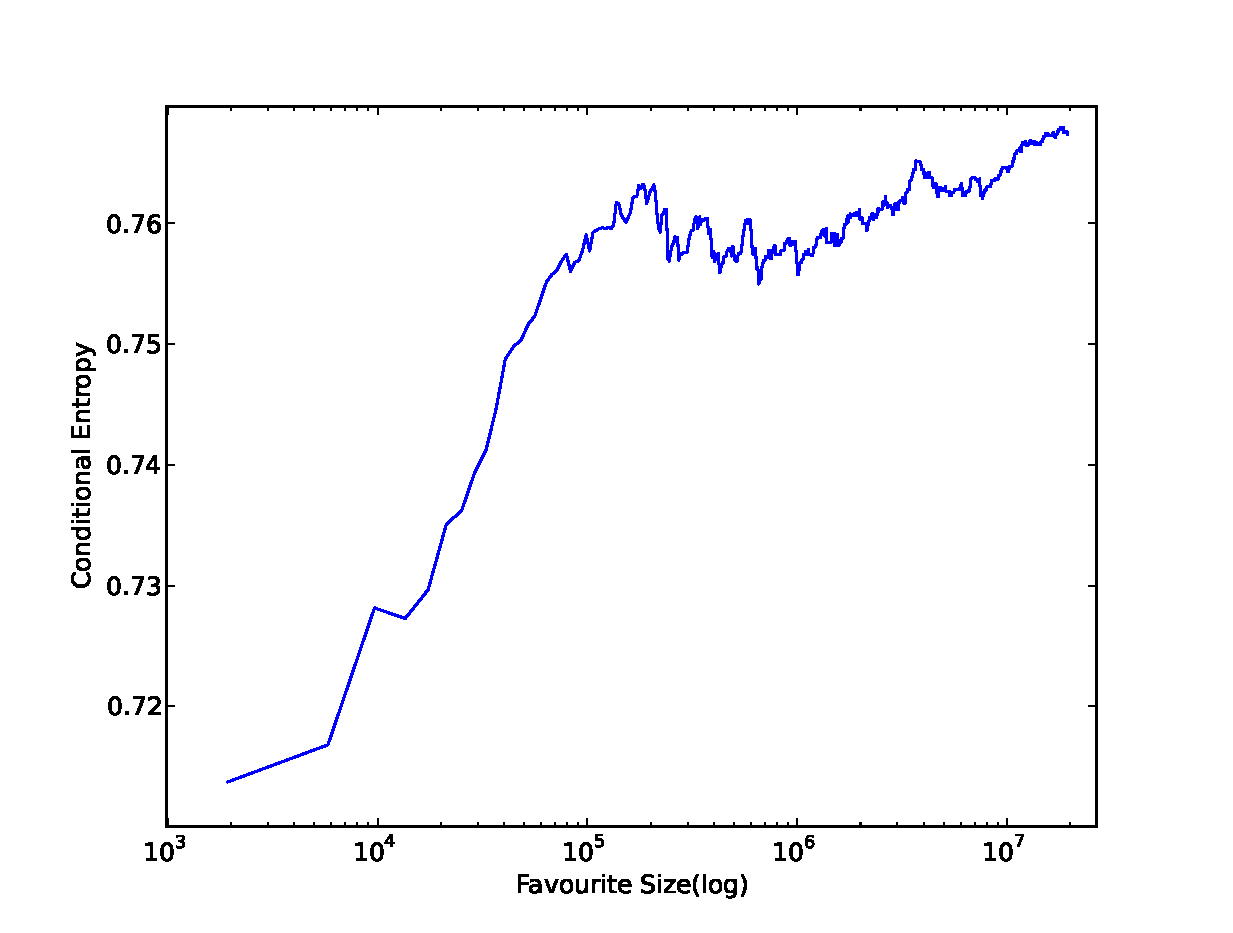
\includegraphics[scale=0.25]{data/plots/cumulativeEntropy/CEvsFavSize_Top800Features_5000bins.eps}}
\end{tabular}
\caption{Average conditional entropy of top 10\% groups, pages and favourites features cumulative over the size }
\label{Fig4}
\end{figure*}
%%%%%%%%%%%%%%%%%%%%%%%%%%%%%%%%%%%%%%%%%%%%%%%%%%%%%%%%%%%%%%%%%%%%%%%%%%%

%%%%%%%%%%%%%%%%%%%%%%%%%%%%%%%%%%%%%%%%%%%%%%%%%%%%%%%%%%%%%%%%%%%%%%%%%%%
\begin{figure*}
\centering
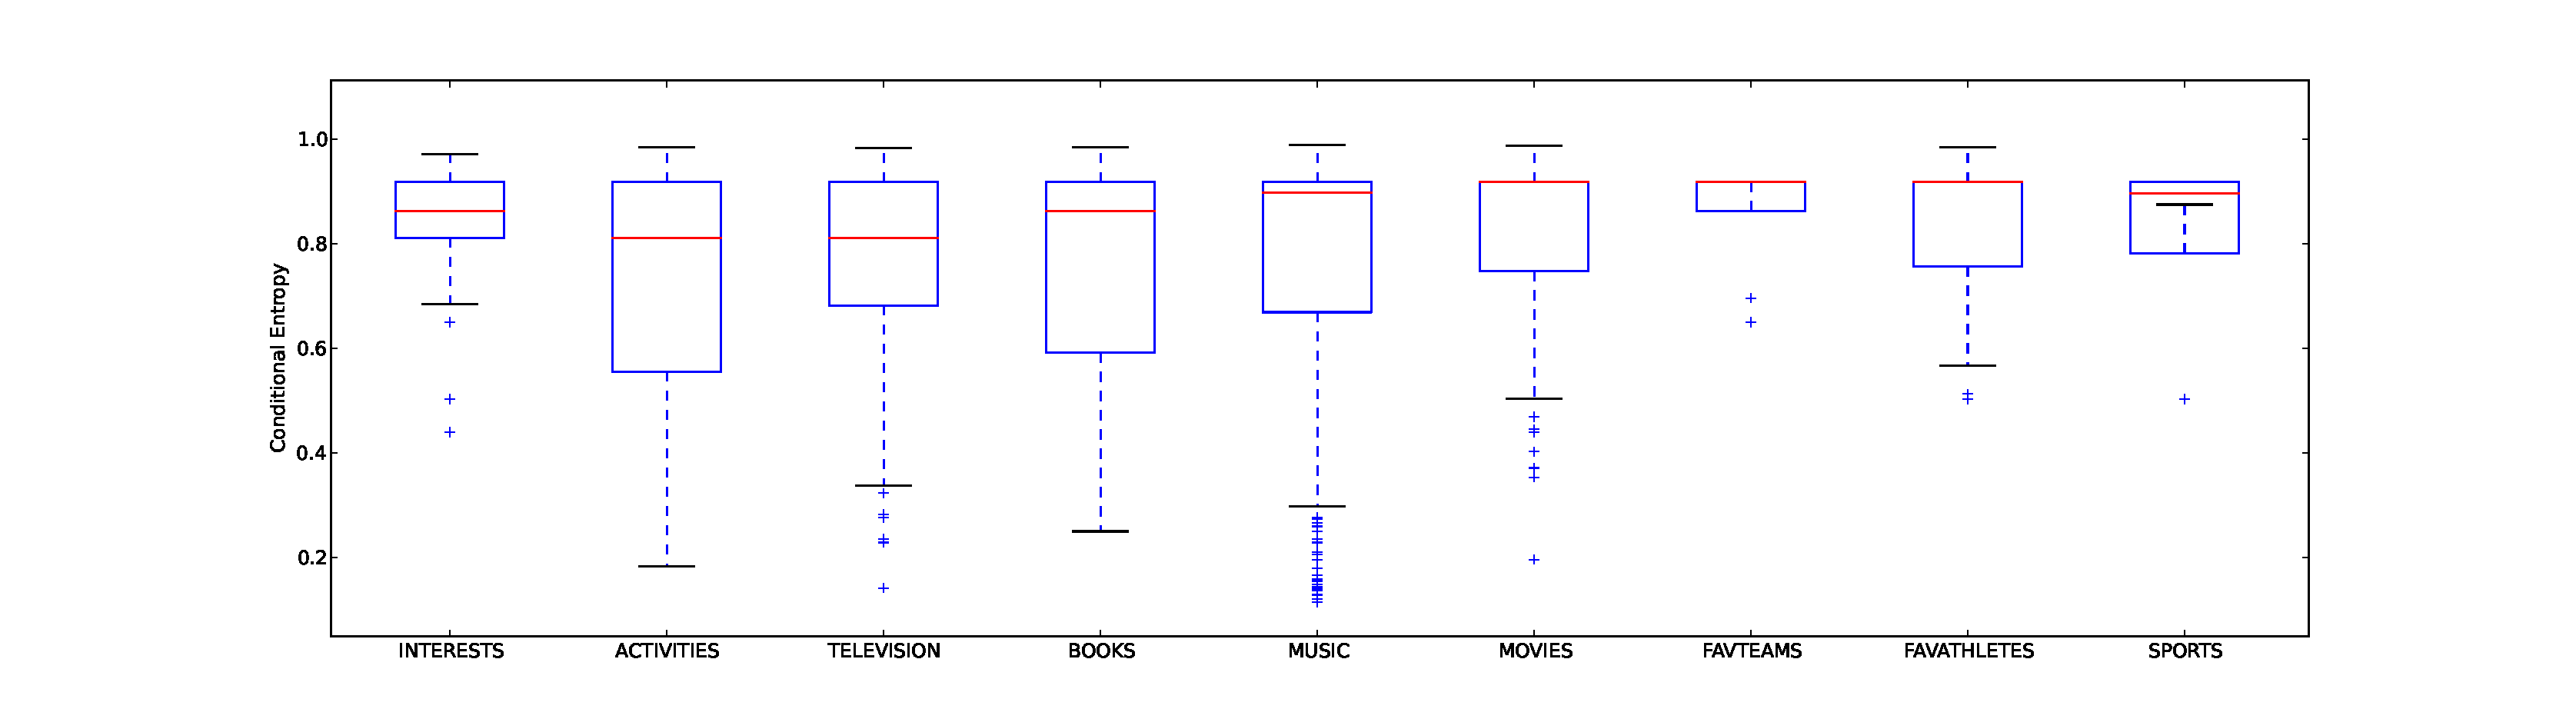
\includegraphics[width=180mm, height=40mm]{data/plots/boxPlots/CEvsFavTypes.eps}
\caption{Conditional entropy for top 1000 favourites breakdown by categories}
\label{Fig5}
\end{figure*}
%%%%%%%%%%%%%%%%%%%%%%%%%%%%%%%%%%%%%%%%%%%%%%%%%%%%%%%%%%%%%%%%%%%%%%%%%%%
